The web services framework is used to expose business services in a
technology-neutral way over some network, which in most cases is the public
Internet.  Wrapping business services in a technology-neutral layer allows
one to decouple the front-end technologies, specifically the user interface
technologies from the back-end technologies, it also allows for the decoupling
of back-end services from one another, in effect communication between dispate
applications.  This decoupling provides one with the ability to vary either the
front-end technologies and back-end technologies independantly from one
another.  Furthmore this allows one to write back-end servies in the most
appropriate technology stack and then have seamless communication between these
indiivdual components.

\subsection{Architecture Requirements}
The architectural requirements for the web service framework include the
refined quality requirements and architectural requirements listed below. The
architectural constraints for this lower level components are the same as for
the system as whole, as referred to in section \ref{sec:systemArchitecturalConstraints}
with further extensions as specified in section \ref{sec:persistenceAPIArchitecturalConstraints}.

\subsubsection{Access and Integration Requirements}
\subsubsection{Quality Requirements}
\paragraph{Maintainability}
\label{sec:webServicesFrameworkMaintainability}
The web services framework is concerned with wrapping business logic, thereby
allowing one to categorize this as so called "plumbing code" which should be as
far as possible be removed from the actual code. This code is normally applied
by the use of annotations in the Java context or by weaving the code into
existing business code using aspects.

Using the above mentioned approach allows one more easily to maintain the code
base.

\paragraph{Integrability}
The framework should enable one to expose business services in a technology
neutral way to allow for easy integration with other independant business
services and systems.  The chosen technology neutral format should be supported
by the business services and system that require integration.

\subsubsection{Architectural Responsibilities}
The architectural responsibilities of the Web Services Framework are shown in 
Figure \ref{fig:webServicesFrameworkResponsibilities}
\begin{figure}[H]
	\begin{center}
	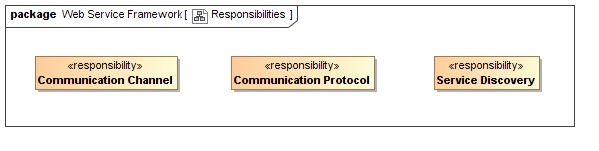
\includegraphics[scale=0.5]{../Diagrams and Charts/Web Services Framework/Responsibilities.jpg}
	\caption{The architectural responsibilities of the Web Services Framework}
	\label{fig:webServicesFrameworkResponsibilities}
	\end{center}
\end{figure}

\subsubsection{Architecture Constraints}
The chosen persistence API should be a currently active standard, with a medium
to large sized active community supporting the standard and should be realized
by at least three active realizations of the chosen API as to ensure future 
maintainability as setout by the required quality requirement in 
section \ref{sec:webServicesFrameworkMaintainability}.

\subsection{Architecture Design}
\subsubsection{Tactics}
The Web Services Framework implement the following tactics:
\paragraph{Support Communication Channels}
The web services framework should support the communication channel to be used
between the client and server as well as between between business services.
With regards to this project the communication channels will consists of a
standards based network connection between all parties, with the communication
channel not necessarily being uniform between all parties. The most likely
communication channel between the client and server will be the Internet
network with a internet network between business services.

\paragraph{Support Standard Communication Protocols}
The web service framework should support standards based communication
protocols as this will ensure the highest change of ensuring full
integrability between client and other business services. All parties should
at least support one of the standards the selected web services framework
supports, thereby ensuring all parties will have successfull communication.

\paragraph{Dynamic Service Discovery}
The provided web services framework should allow for dynamic service discovery
by the clients with the clients only knowing where to locate the root service.
This will ensure easier maintainability as clients and other services will not
need to be informed with the location of the services have changed.

\subsubsection{Architectural Components}
\subsubsection{Frameworks and Technologies}
\paragraph{Concrete Realization of Architectural Components}
\paragraph{Tactics}
\paragraph{Tools}
\paragraph{Concepts and Constraints for Application Components}